\documentclass[notes]{beamer} % beamer
\usepackage[framesassubsections]{beamerprosper} % beamer
\usepackage{setspace}
\usepackage{textpos}
\usepackage{wrapfig} % bilder von text umfliessend
\usepackage{hyperref} % url
\usepackage{listings} % code
\usepackage[german]{babel} %sprache
\usepackage[latin1]{inputenc} %codierung

%\setbeamertemplate{footline}[page number]
%\setcounter{tocdepth}{1}
%\setbeameroption{show only notes}
%\setbeameroption{hide notes}
%%%%%%%%%%%%%%%%%%%%%%%%%%%%%%%%%%%%%%%%%%%%%%
% Titel
\title{EERT}
\subtitle{OpenGL mit Java (WS 08/09)}
\author{ Robert Schadek}
\date{25. Febuar 2009}
\institution{Department f\"ur Informatik, Universit\"at Oldenburg }

\begin{document}
\maketitle
%%%%%%%%%%%%%%%%%%%%%%%%%%%%%%%%%%%%%%%%%%%%%%
\begin{frame}
\begin{spacing}{1}
\frametitle{Gliederung}
\tableofcontents[hidesubsections]
\end{spacing}
\end{frame}
%%%%%%%%%%%%%%%%%%%%%%%%%%%%%%%%%%%%%%%%%%%%%%
\section{Motivation}
\begin{frame}
\begin{spacing}{1}
\frametitle{Motivationa}
\begin{itemize}
\item flexibel durch Szenefiles
\item unbeschr"ankt durch Objektloader
\item einfaches schnelles texturieren
\item hohe Performance
\end{itemize}
\end{spacing}
\end{frame}
%%%%%%%%%%%%%%%%%%%%%%%%%%%%%%%%%%%%%%%%%%%%%%
\section{Techniken}
\begin{frame}
\begin{spacing}{1}
\frametitle{Techniken}
\begin{itemize}
\item Directional Per-Fragment Lightning
\item .obj Loader
\item Quadratische B\'{e}zierkurven
\item Objektinstanzen
\item Level of Detail
\item Octree Frustum Culling
\end{itemize}
\end{spacing}
\end{frame}
%%%%%%%%%%%%%%%%%%%%%%%%%%%%%%%%%%%%%%%%%%%
\section{Quadratische B\'{e}zierkurven}
\begin{frame}
\begin{spacing}{1}
\frametitle{Quadratische B\'{e}zierkurven}
\begin{itemize}
\item wird benutzt um Kamera-flug zu simulieren
\item nicht FPS abh"angig
\item Formel $(1-t)^{2}P_{0} + 2t(1-t)P_{1} + t^{2}P_{2}$ $t \in [0,1]$
\item $t = 1 - timer / timeSlice$ 
\item timeSlice gibt an wie lange es dauert die Kurve abzulaufen
\item zwei Kurven eine f"ur Kameraposition eine f"ur Blickpunkt
\end{itemize}
\end{spacing}
\end{frame}

%%%%%%%%%%%%%%%%%%%%%%%%%%%%%%%%%%%%%%%%%%%
\section{Objektinstanzen}
\begin{frame}
\begin{spacing}{1}
\frametitle{Objektinstanzen}
\begin{itemize}
\item Ziel ist Speicherplatz sparen
\item Mesh wird einmal geladen und als DisplayList gespeichert
\item beliebig viele Objektinstanzen werden zum Mesh erstellt
\item Objektinstanz muss prinzipell nur Position und Rotation speicher
\item Suzann 1.3MB gro"s 400mal in Szene $=$ 520MB auf Grafikkarte
\item Mit Objektinstanzen 1.3MB auf Grafikkarte
\end{itemize}
\end{spacing}
\end{frame}

%%%%%%%%%%%%%%%%%%%%%%%%%%%%%%%%%%%%%%%%%%%
\section{Level of Detail}
\begin{frame}
\begin{spacing}{1}
\frametitle{Level of Detail}
\begin{itemize}
\item entfernte Objekte brauchen nicht max. Detailgrad
\item Grundform gen"ugt
\item EERT sechs Aufl"osungen f"ur jedes Objekt
\item reduziert Anzahl Dreicke von ca. 4 Million auf wenige 10000
\item ohne das dies st"orend auff"allt
\item Level wird anhand der Distanz zur Kameraposition ausgew"ahlt
\end{itemize}
\end{spacing}
\end{frame}
%%%%%%%%%%%%%%%%%%%%%%%%%%%%%%%%%%%%%%%%%%%%
\section{Octree}
\begin{frame}
\begin{spacing}{1}
\frametitle{Octree}
\begin{itemize}
\item Raumaufteilung f"ur Frustum Culling
\item Baumstruktur mit je acht Unterknoten
\item Raum wird durch Ebenen Achsen geteilt
\item jeder Raum enth"allt Liste von Objekten die sich in ihm befinden
\item nur in den Bl"attern wird gezeichnet
\item wenn Knoten nicht im Frustum $\rightarrow$ kein Kind sichtbar
\item Anzahl der Knoten w"achst mit $8^{n}$ wobei $n = Baumtiefe$
\item Rekursiv implementierbar
\item EERT $Baumtiefe = 4$ also maximal 4096 Knoten
\end{itemize}
\end{spacing}
\end{frame}

\begin{frame}
\begin{spacing}{1}
\frametitle{Octree Aufbau}
\begin{enumerate}
\item Mittelpunkt und Ausdehnung der Szene bestimmen
\item Ersten Unterknoten bestimmen 
\item Objekte Bestimmen die in ihm liegen
\item Unterknoten aufteilen usw. bis max. Tiefe erreicht
\item n"achsten Unterknoten und dessen Unterknoten erstellen
\end{enumerate}

\begin{itemize}
\item leere Unterknoten werden verworfen und nicht weiter abgestiegen
\item Aufbau bei 400 Objekte unterhalb 2ms
\end{itemize}
\end{spacing}
\end{frame}

\begin{frame}
\begin{spacing}{1}
\frametitle{Aufgebauter Octree}
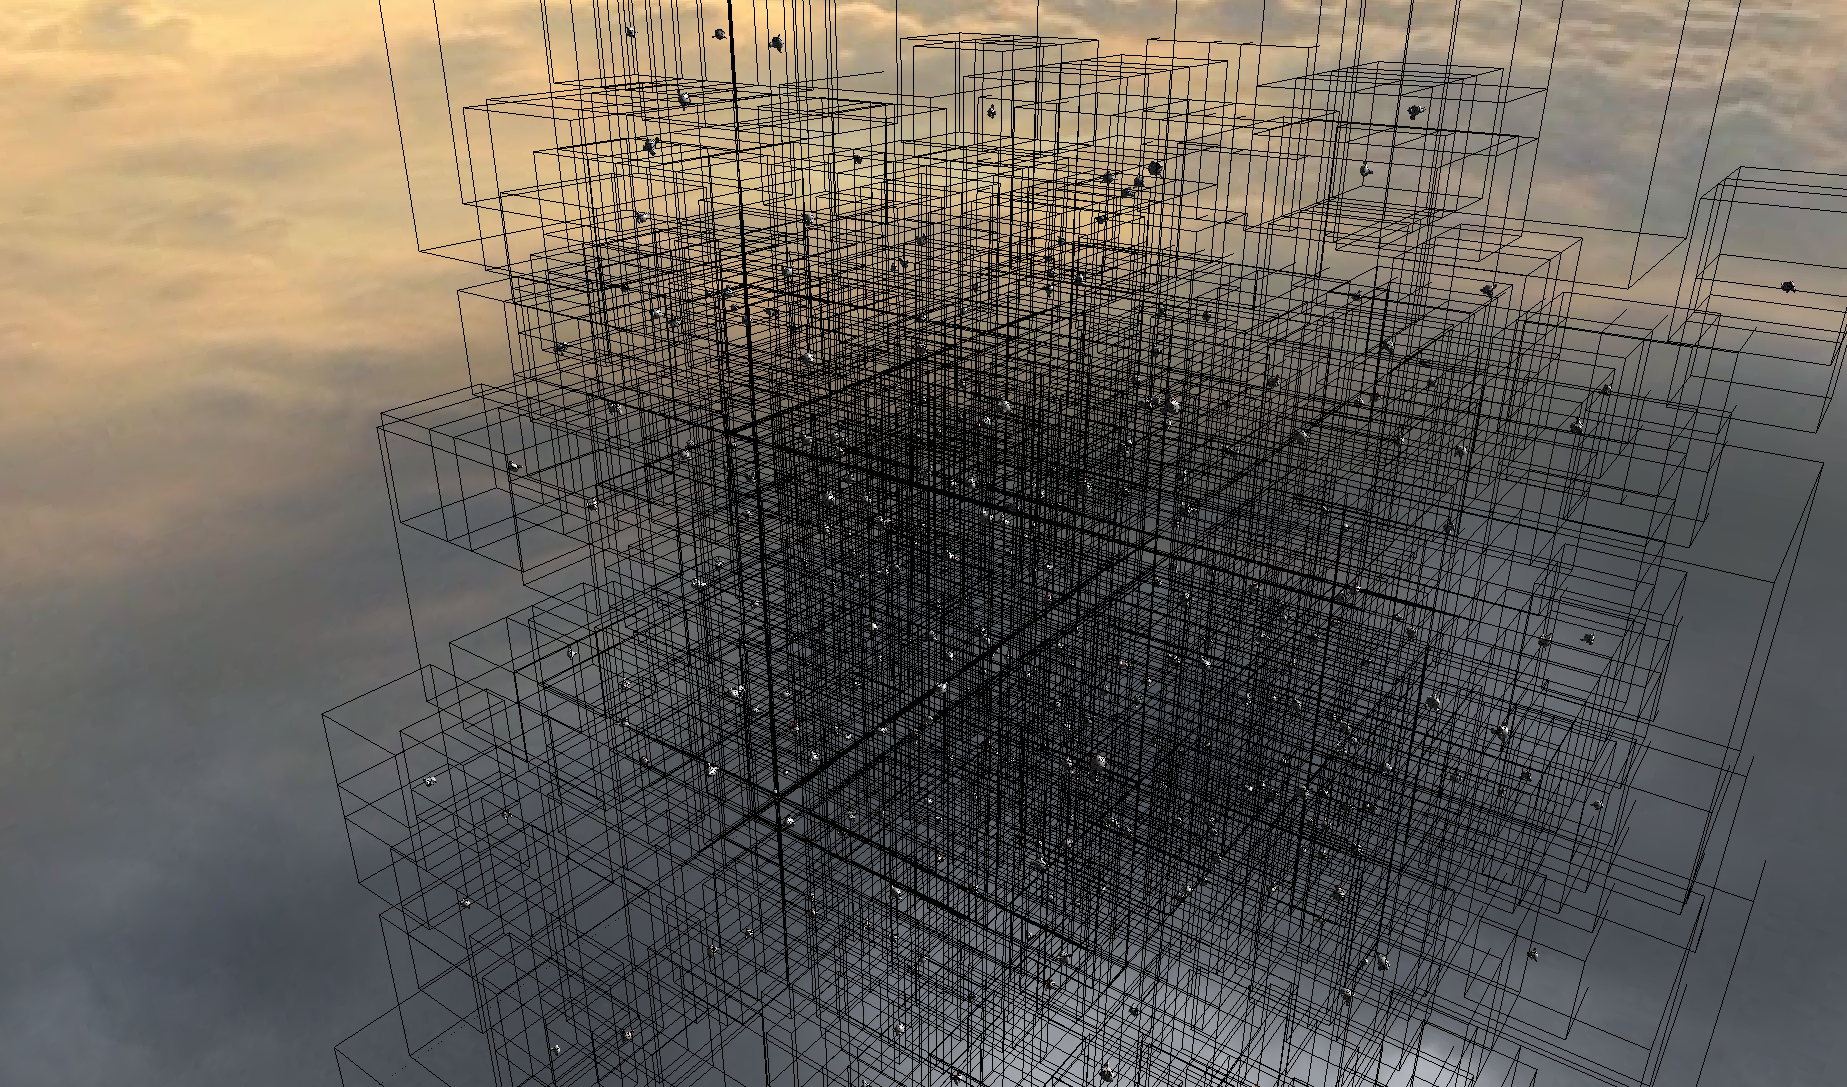
\includegraphics[width = 1.0\textwidth]{oc2.png}
\end{spacing}
\end{frame}

\begin{frame}
\begin{spacing}{1}
\frametitle{Zeichen Octree}
\begin{enumerate}
\item pr"ufen ob Wurzel im Frustum\\wenn nicht fertig
\item pr"ufen ob erstes Kind im Frustum\\wenn nicht n"achstes Kind
\item wiederhole Schritt zwei bis Kind $=$ Blatt alle Objekte im Kind zeichnen
\end{enumerate}
\end{spacing}
\end{frame}

%%%%%%%%%%%%%%%%%%%%%%%%%%%%%%%%%%%%%%%%%%%%%%%%%%
\section{Fragen}
\begin{frame}
\begin{center}
Fragen?
\end{center}
\end{frame}

\end{document}
